\documentclass{article}
\usepackage[margin=1in]{geometry}
\usepackage{amsmath}
\usepackage{graphicx}
\usepackage{caption}
\usepackage{float}
\usepackage{tikz}
\usetikzlibrary{arrows,calc}

\title{MATH 367 Assignment}
\date{2017-04-01}
\author{Ian McKenzie, Scott Nerbas}

\begin{document}
\pagenumbering{gobble}
\maketitle
\newpage
\pagenumbering{arabic}

\section{Exercise 1}
Provide justifications for the first four assumptions.
\subsection{}
The first assumption is probably reasonable for small populations.
Obviously it cannot hold in real life for arbitrarily large populations, as resources such as rabbit food are scarce in nature.
\subsection{}
The rabbits being eaten at a rate proportional to the size of both rabbit and wolf
populations seems reasonable.
Immortal rabbits seems a bit odd at first, but when the wolf population is large enough compared to the rabbit population it seems likely that the only source of rabbit deaths would be being eaten by wolves.
\subsection{}
Rabbits being the only source of food for wolves seems reasonable considering the nature of the small island and assuming that there are only 2 species on the entire island.
\subsection{}
Mortal wolves seems to approximate real life very well, however a more sophisticated model would likely take into account disease or other predators.

\section{Exercise 2}
Suppose $x(t)=0$ for all $t$. What is $y(t)$? Suppose $y(t)=0$ for all $t$. What is $x(t)$?
Are these answers reasonable?
\subsection{}
When $x(t)=0$,
\begin{align*}
  y'(t) &= -d~y(t) \\
  \frac{y'(t)}{y(t)} &= -d \\
  \int \frac{y'(t)}{y(t)}~dt &= \int -d~dt \\
  &\setbox0\hbox{=}\mathrel{\makebox[\wd0]{\hfil\vdots\hfil}} \\
  y(t) &= k~e^{-dt} \\
\end{align*}
where $k$ is some constant.
\subsection{}
When $y(t)=0$,
\begin{align*}
  x'(t) &= a~x(t) \\
  \frac{x'(t)}{x(t)} &= a \\
  \int \frac{x'(t)}{x(t)}~dt &= \int a~dt \\
  &\setbox0\hbox{=}\mathrel{\makebox[\wd0]{\hfil\vdots\hfil}} \\
  x(t) &= k~e^{at} \\
\end{align*}
where $k$ is some constant.

\section{Exercise 3}
\subsection{}
If $x(t)\geq 0$ and $x'(t)=0$ then $0=x(t)~(a-by(t))$. This means that $a-by(t)$ must be 0, so:
\begin{equation*}
  y(t) = \frac{a}{b}
\end{equation*}
If $y(t)\geq 0$ and $y'(t)=0$ then $0=y(t)~(cx(t)-d)$. This means that $cx(t)-d$ must be 0, so:
\begin{equation*}
  x(t) = \frac{d}{c}
\end{equation*}
\subsection{}
Parametric population trajectory curves are indicated by arrows. \\
\begin{center}
\begin{tikzpicture}[scale=0.5,>=latex]
  \coordinate (y) at (0,12);
  \coordinate (x) at (12,0);
  \draw[<->] (y) -- (0,0) -- (x);
  \coordinate (cd) at ($0.5*(x)$);
  \coordinate (ab) at ($0.5*(y)$);
  \draw[dashed,thick] let \p1=(cd), \p2=(y) in
  (\p1) node[below] {$\frac{d}{c}$} -- (6,12);
  \draw[dashed,thick] let \p1=(ab), \p2=(x) in
  (\p1) node[left] {$\frac{a}{b}$} -- (12,6);
  \draw[->] (3,5) -- (5,3);
  \node at (2,2) {$R_{+-}$};
  \draw[->] (7,3) -- (9,5);
  \node at (10,2) {$R_{++}$};
  \draw[->] (9,7) -- (7,9);
  \node at (10,10) {$R_{-+}$};
  \draw[->] (5,9) -- (3,7);
  \node at (2,10) {$R_{--}$};
\end{tikzpicture}
\end{center}

\newpage
\section{Excersize 4}
By first order approximation,
\begin{equation*}
  y(t_1) = y(t_0 + \Delta t) \approx y(t_0) + y'(t_0)\Delta t = y_0+y'(t_0)\Delta t
\end{equation*}
and,
\begin{equation*}
  y'(t_0) = cx(t_0)y(t_0) - dy(t_0) = cx_0y_0 -dy_0.
\end{equation*}
Therefore,
\begin{equation*}
  y(t_1) = y(t_0 + \Delta t) \approx y_0 + (cx_0y_0 - dy_0)\Delta t.
\end{equation*}

\section{Exercise 5}
\centerline{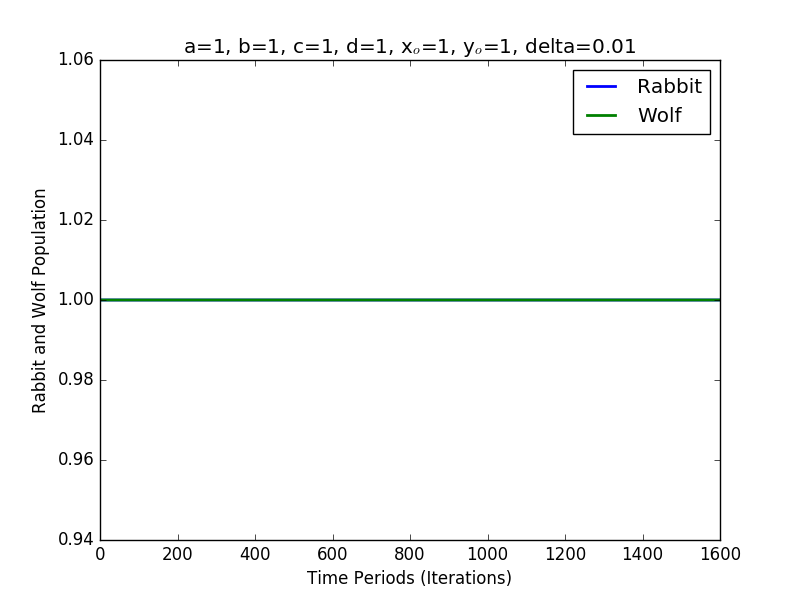
\includegraphics[scale=0.5]{exercise5/figure_1.png}}
In this simulation, we used the constants $a, b, c, d$ all equal to 1.
The starting population values are both 1.
The populations do not grow or decline from their initial values.\\

\newpage
\centerline{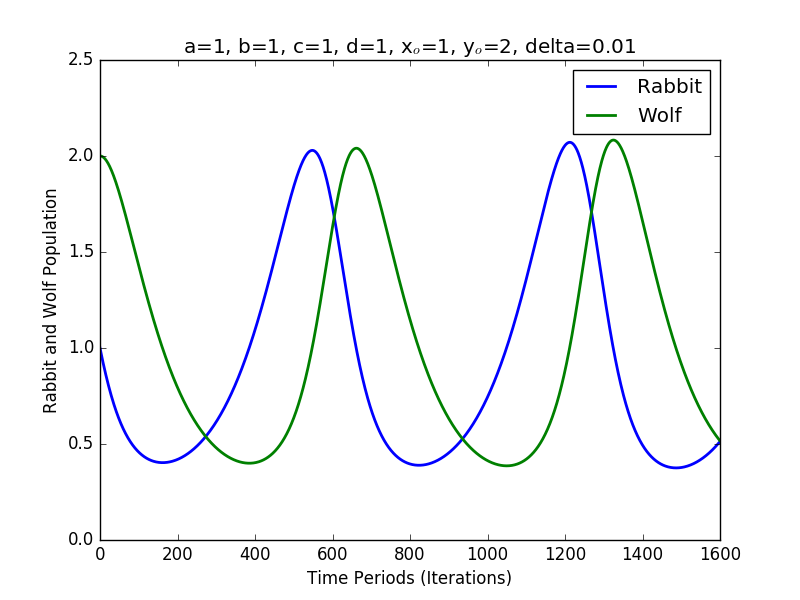
\includegraphics[scale=0.5]{exercise5/figure_1-6.png}}
In this simulation, we used the constants $a, b, c, d$ all equal to 1.
The starting population values are $x_0=1$ for rabbits and $y_0=2$ for wolves.
The rabbit and the wolf functions appear to have the same maximums and minimum values in this case.\\
\centerline{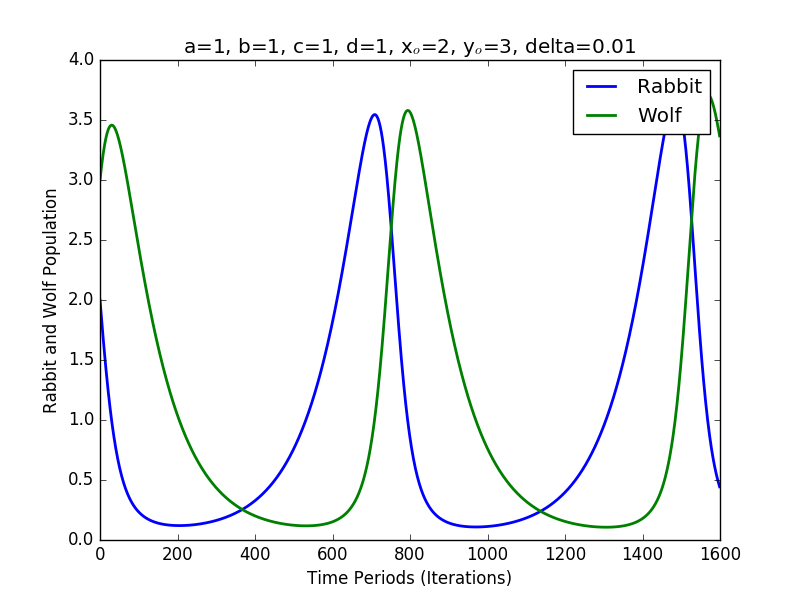
\includegraphics[scale=0.5]{exercise5/figure_1-1.png}}
In this simulation, we used the constants $a, b, c, d$ all equal to 1.
The starting population values are $x_0=2$ for rabbits and $y_0=3$ for wolves.
The rabbit function appears to have a higher maximum than the wolf function, and the wolf function appears to have the same minimum value as the rabbit function.
Furthermore, the functions appear to be mirror images of each other.\\
\\
\centerline{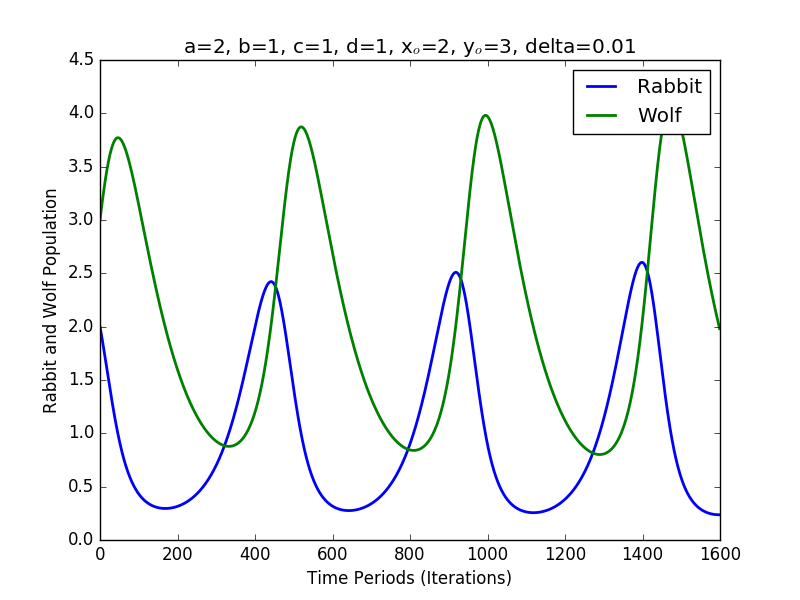
\includegraphics[scale=0.5]{exercise5/figure_1-2.png}}
In this simulation, we used the constants $a=2, b=1, c=1, d=1$ and starting population values of $x_0=2$ and $y_0=3$.
The wolf function appears to have a higher maximum and minimum than the rabbit function.\\
\\
\centerline{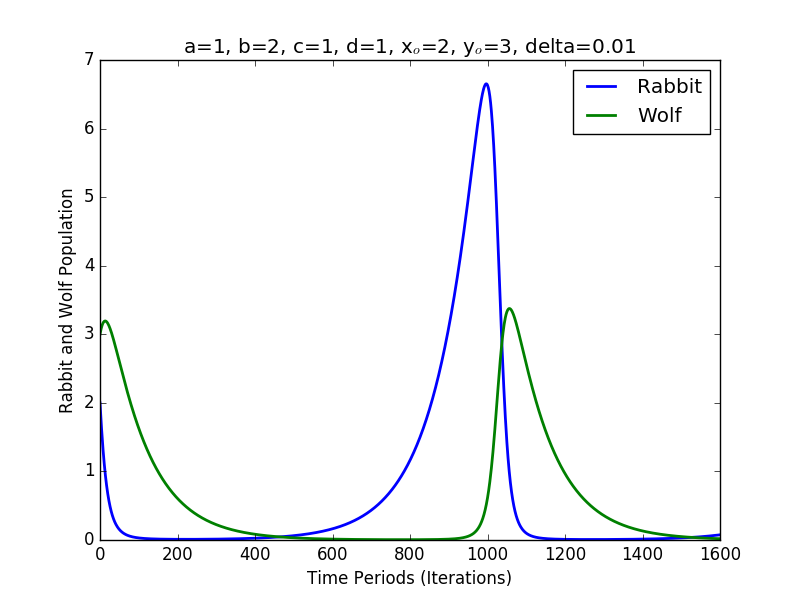
\includegraphics[scale=0.5]{exercise5/figure_1-3.png}}
In this simulation, we used the constants $a=1, b=2, c=1, d=1$ and starting population values of $x+0=2$ and $y_0=3$.
The rabbit population dramatically increases in size before collapsing as he wolf population increases.\\
\\
\centerline{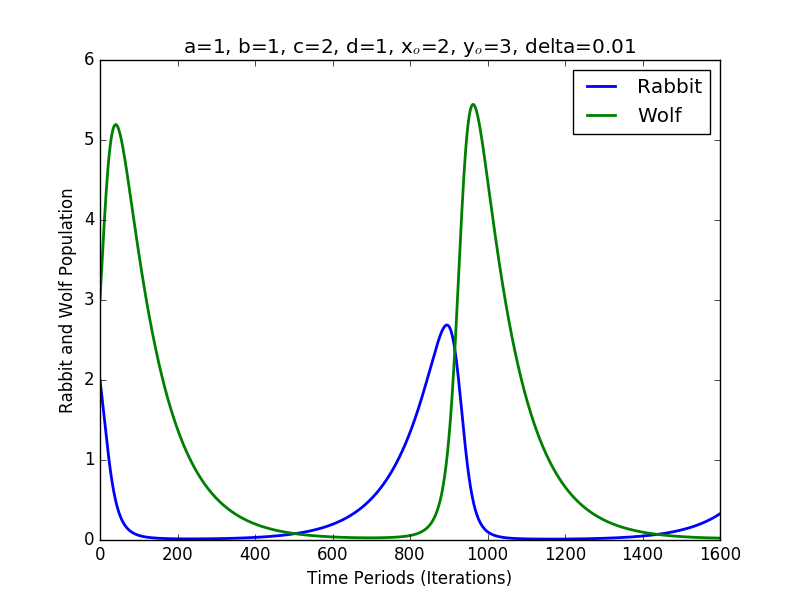
\includegraphics[scale=0.5]{exercise5/figure_1-4.png}}
In this simulation, we used the constants $a=1, b=1, c=2, d=1$ and starting population values of $x_0=2$ and $y_0=3$.
As the wolf population suddenly decreases, the rabbit population rapidly rises.\\
\\
\centerline{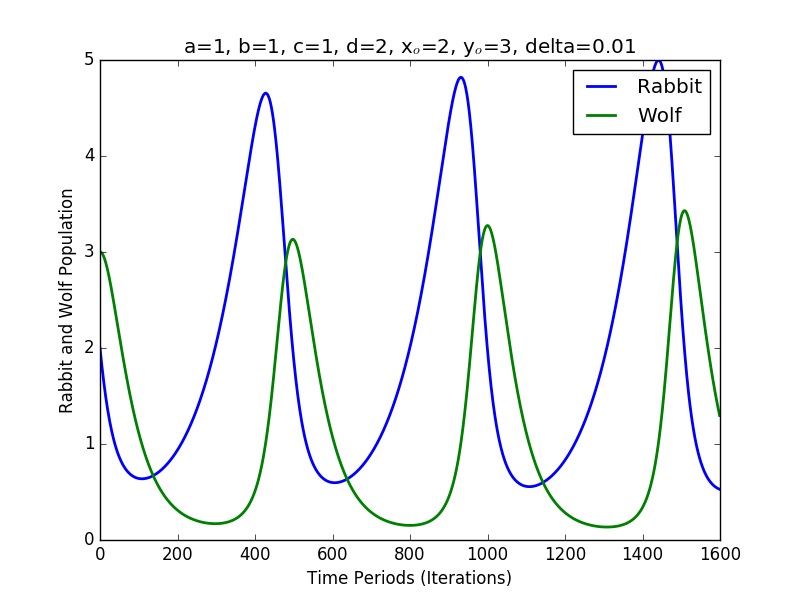
\includegraphics[scale=0.5]{exercise5/figure_1-5.png}}
In this simulation, we used the constants $a=1, b=1, c=1, d=2$.
The starting population values are $x_0=2$ and $y_0=3$.
The rabbit function appears to have a higher maximum and minimum than the wolf function.\\

\section{Exercise 6}
We used initial population values of $x_0=2$, $y_0=1$.
We use the gradient descent algorithm for minimization.
\subsection{$(a,b)$}
The gradient of the $(a,b)$ error function is:
\begin{equation*}
  \nabla E_{a,b}=
  \left (
    \sum_{k=1}^{n}-2x_k\Big(\frac{x_k-x_{k-1}}{t_k-t_{k-1}}-(ax_k - bx_ky_k)\Big),
    \sum_{k=1}^{n}2x_ky_k\Big(\frac{x_k-x_{k-1}}{t_k-t_{k-1}}-(ax_k - bx_ky_k)\Big)
  \right )
\end{equation*}\\
To avoid local minimums, we first plot the error function so we can start our gradient descent near the absolute minimum.
\\
\begin{figure}[H]
  \centering
  \begin{minipage}[t]{0.49\textwidth}
    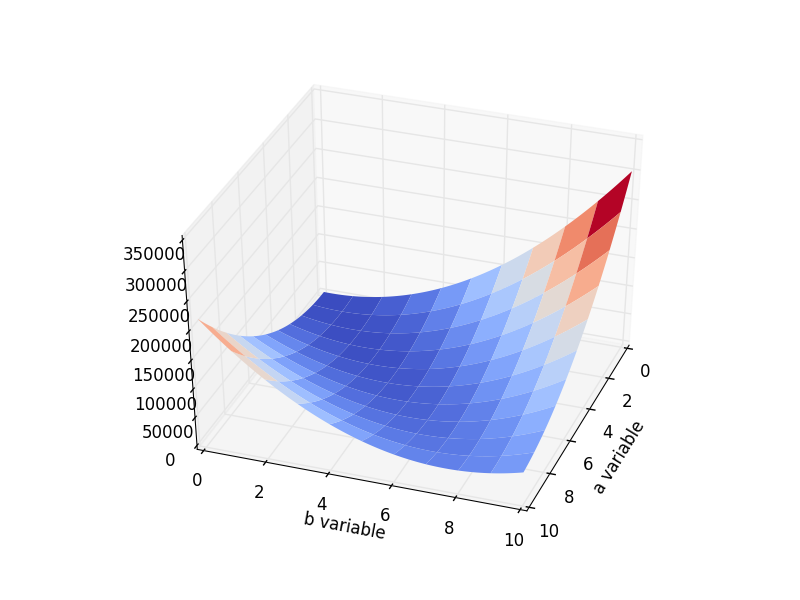
\includegraphics[width=\textwidth]{exercise6/ab_error_big.png}
    \caption*{Large plot.}
  \end{minipage}
  \begin{minipage}[t]{0.49\textwidth}
    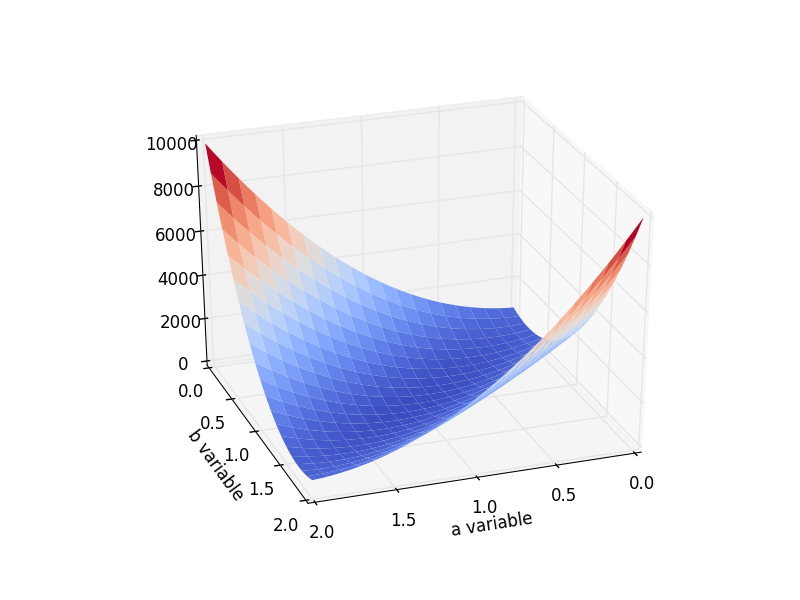
\includegraphics[width=\textwidth]{exercise6/ab_error_small.png}
    \caption*{Near origin.}
  \end{minipage}
\end{figure}
From this it appears that the minimum is near the origin, so we produce another plot with less range to illuminate the area near the origin.
From this second plot it seems that the minimum occurs near the point $a=b=1$, so we begin our gradient descent at that point.
\\
\begin{figure}[H]
  \centering
  \begin{minipage}[t]{0.49\textwidth}
    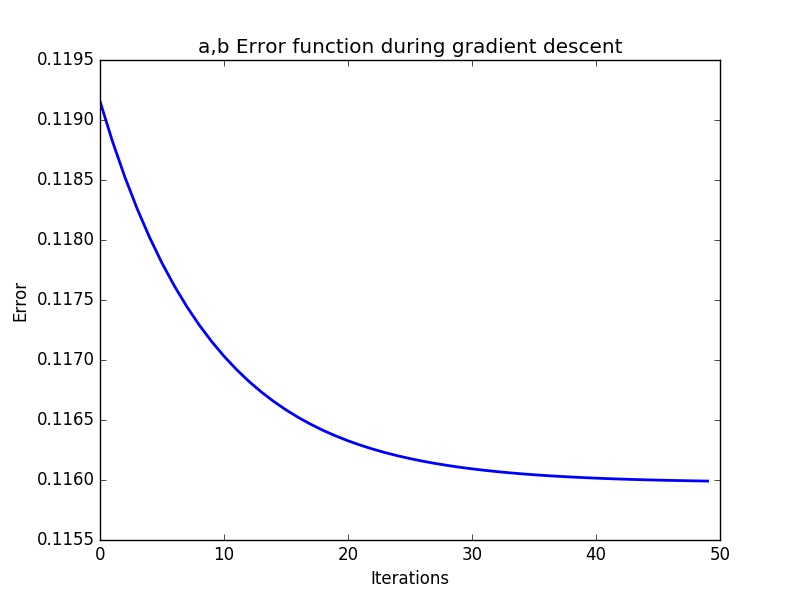
\includegraphics[width=\textwidth]{exercise6/ab_descent_illustration.png}
    \caption*{50 iterations, larger $\Delta$.}
  \end{minipage}
  \begin{minipage}[t]{0.49\textwidth}
    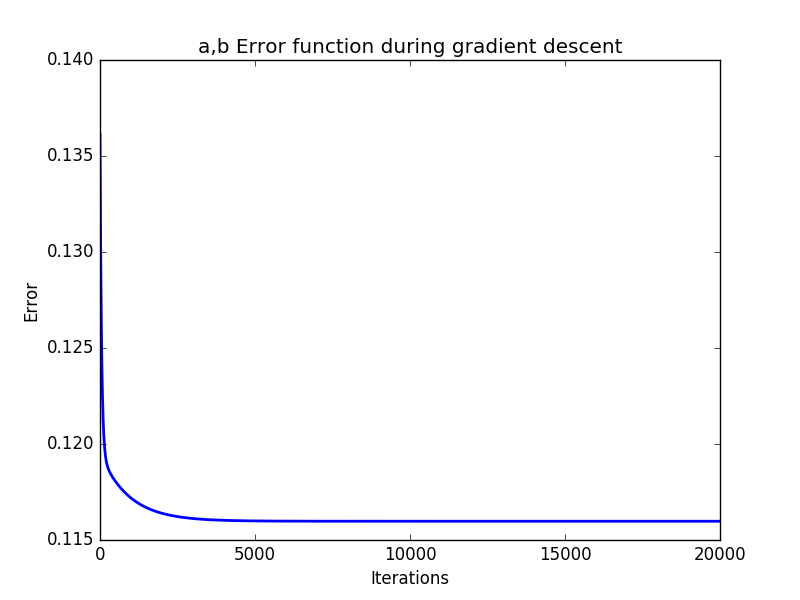
\includegraphics[width=\textwidth]{exercise6/ab_descent_actual.png}
    \caption*{Actual convergence. 20,000 iterations, smaller $\Delta$.}
  \end{minipage}
\end{figure}
To illustrate how our gradient descent converges, we show the error over 50 iterations with a step size of 0.0001.
To find a more accurate minimum, we computed 20,000 iterations with a step size of 0.000001.
This resulted in the minimum of 0.11598 which occurs at $a=1.00398, b=1.00084$.
From the actual convergence plot, we can see that 20,000 iterations is probably excessive, but at least we know that the minimum is accurate.
\subsection{$(c,d)$}
The gradient of the $(c,d)$ error function is:
\begin{equation*}
  \nabla E_{c,d}=
  \left (
    \sum_{k=1}^{n}-2x_ky_k\Big(\frac{y_k-y_{k-1}}{t_k-t_{k-1}}-(cx_ky_k-dy_k)\Big),
    \sum_{k=1}^{n}2y_k\Big(\frac{y_k-y_{k-1}}{t_k-t_{k-1}}-(cx_ky_k-dy_k)\Big)
  \right )
\end{equation*}\\
Again, to avoid local minimums, we first plot the error functions so we can start our gradient descent near the absolute minimum.
\\
\begin{figure}[H]
  \centering
  \begin{minipage}[t]{0.49\textwidth}
    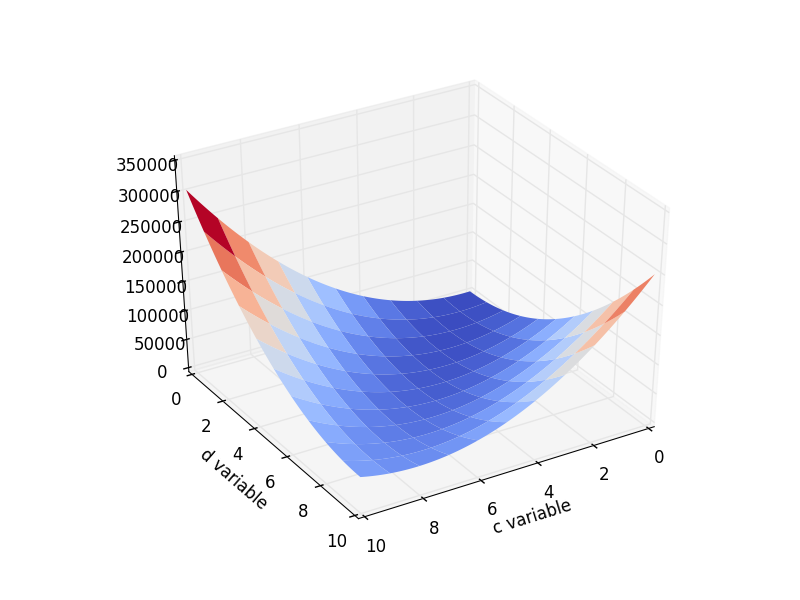
\includegraphics[width=\textwidth]{exercise6/cd_error_big.png}
    \caption*{Large plot.}
  \end{minipage}
  \begin{minipage}[t]{0.49\textwidth}
    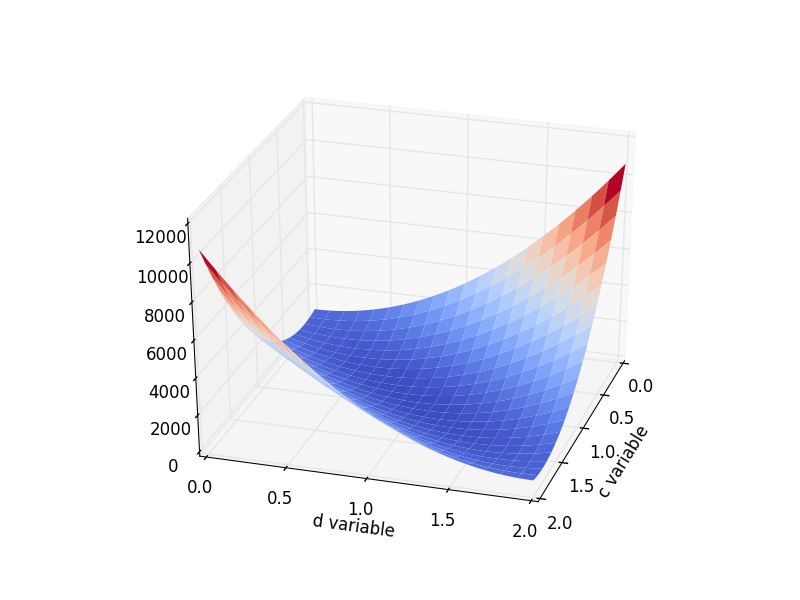
\includegraphics[width=\textwidth]{exercise6/cd_error_small.png}
    \caption*{Near origin.}
  \end{minipage}
\end{figure}
From this it appears that the minimum occurs near the origin, so we produced another plot with less range to illuminate the area near the origin.
From this second plot it seems that the minimum occurs near the point $c=d=1$, so we begin out gradient descent at that point.
\\
\begin{figure}[H]
  \centering
  \begin{minipage}[t]{0.49\textwidth}
    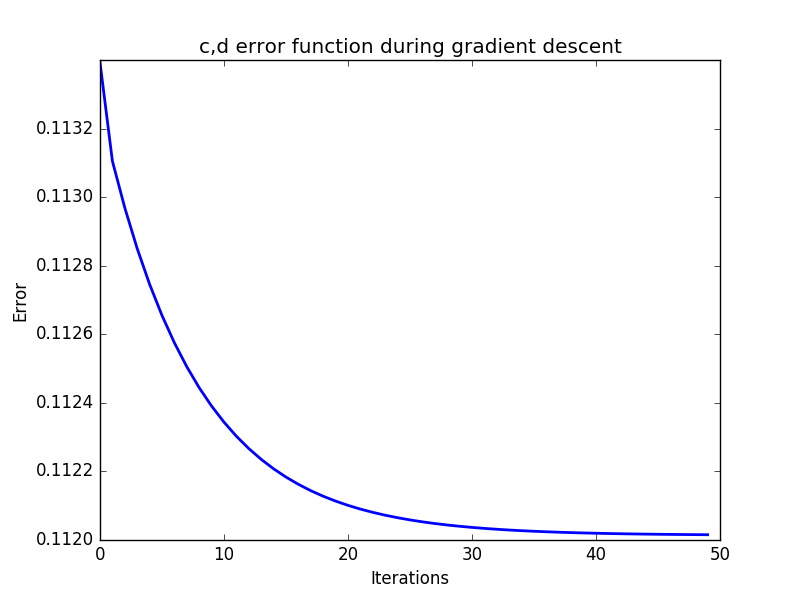
\includegraphics[width=\textwidth]{exercise6/cd_descent_illustration.png}
    \caption*{50 iterations, larger $\Delta$.}
  \end{minipage}
  \begin{minipage}[t]{0.49\textwidth}
    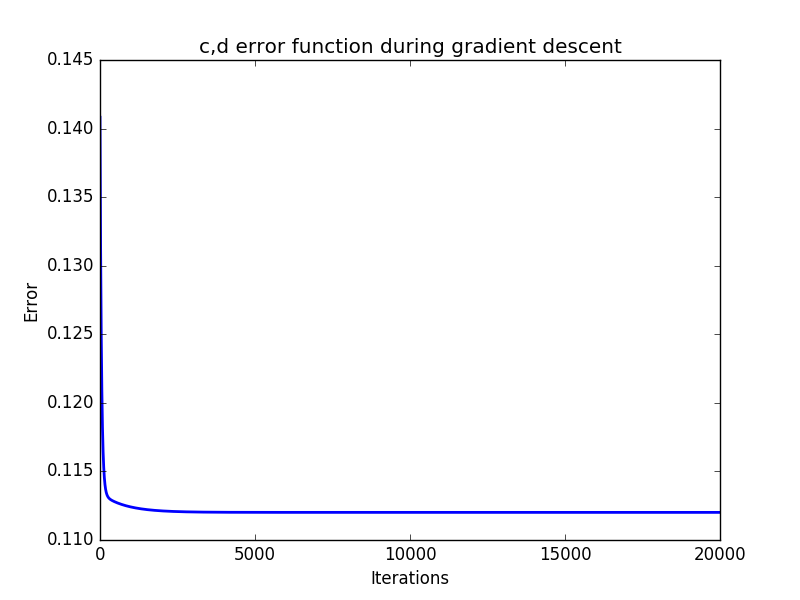
\includegraphics[width=\textwidth]{exercise6/cd_descent_actual.png}
    \caption*{Actual convergence. 20,000 iterations, smaller $\Delta$.}
  \end{minipage}
\end{figure}
To illustrate how our gradient descent converges, we show the error over 50 iterations with with a step size of 0.0001.
To find a more accurate minimum, we completed 20,000 iterations with a step size of 0.000001.
This resulted in the minimum of 0.11201 which occurs at $c=1.00034, d=0.99691$.
From the plot we can see that 20,000 iterations is probably excessive, but at least we know that the minimum is accurate.\\

\end{document}
%%% Local Variables:
%%% mode: latex
%%% TeX-master: t
%%% End:
